% !TEX Program = xelatex
\documentclass[nonprint, doctor, vlined]{DissertUESTC}


\begin{document}
	
	\definecolor{shadcolor}{RGB}{228, 234, 246}
	\newcommand{\shad}[1]{\colorbox{shadcolor}{#1}}
	\newcommand{\shadcmd}[1]{\shad{$\backslash$#1}}
	
	\nocite{*}
	
	% 封面
%	\uestccover{<论文题目>}{<学科专业>}{<学号>}{<作者姓名>}{<指导教师>}{<教师职称>}{<学院>}
	\uestccover{关于我的杀父仇人疑似是名震天下的大侠时该如何报仇}
				{玉女素心剑法}
				{1182000}
				{杨\hspace{1em}过}
				{小龙女}
				{掌\hspace{1em}门}
				{古墓派}
	
	% 中文扉页
	\ClsNum{TN828.6}  % \ClsNum{<分类号>}
	\ClsLv{公开}  % \ClsLv{<密级>}
	\UDC{621.39}  % \UDC{<UDC号>}
	\DissertationTitle{关于我的杀父仇人疑似是名震天下的大侠时该如何报仇}  % \DissertationTitle{<题名>}
	\Author{杨过}  % \Author{<作者姓名>}
	\Supervisor{小龙女}{掌门}{古墓派}{活死人墓}  % \Supervisor{<指导教师>}{<职称>}{<单位名称>}{<单位地址>}
	% 副导师信息,无则注释
	\AssociateSupervisor{洪七公}{前帮主}{丐帮}{襄阳}  % \AssociateSupervisor{<副导师名称>}{<职称}>{<单位名称>}{<单位地址>}
	\DegLv{西狂}  % \DegLv{<申请学位级别>},该信息由文档类选项自动确定,需修改默认内容时使用,否则注释即可
	\Major{玉女素心剑法}  % \Major{<学科专业>}
	\Profield{剑道}  % \Profield{专业学位领域代码},此为专业学位独有,学术学位用户注释即可
	\Date{1959年1月1日}{1961年1月1日}  % \Date{<论文提交日期>}{<论文答辩日期>}
	\Grant{中华武林}{1961年2月2日}  % \Grant{<学位授予单位>}{<学位授予日期>}
	\Reviewer{黄蓉}{一灯大师、老顽童、黄老邪、郭靖、小龙女}  % \Reviewer{<答辩委员为主席>}{<评阅人>}
	\uestczhtitlepage
	
	% 英文扉页
	% \uestcentitlepage{<文题>}{<专业>}{<学号>}{<作者>}{<导师>}{<副导师>}{<学院>},若无副导师,则将“<副导师>”参数留空即可
	\uestcentitlepage{How to Take Revenge When My Father's Murderer is Suspected to Be a Famous Hero}
					{Jade Lady Soul Sword Technique}
					{1182000}
					{Yang Guo}
					{Grandmaster Dragondaughter Little}{Grandmaster Northern Beggar}
					{Ancient Tomb Sect}
	
	% 独创性声明:[签名宽度]{日期}{作者签名图片}{导师签名图片},送审时使用空强制参数即可
	\declaration[3cm]{2024年08月31日}{authsign}{spvrsign}
	
	% 开启中文摘要
	\zhabstract
	
	杨过少年时期母亲染病而亡,随后他便过着四处流浪的生活。后来遇到郭靖夫妇,便由他们照看。但之后因杨过与郭芙等人之间的矛盾,郭靖便送其去全真派习武。其后,又从全真派逃出,机缘巧合下于古墓遇见小龙女,之后便跟随小龙女练功。 他身边有许多红颜知己钟情于他,而他却一心只爱小龙女,后结为夫妇;他和郭家恩怨难分,数度因误会关系紧张,却始终挺身而出相助他们,解除嫌隙,化气为和;命运多舛,与小龙女分隔十六年里,随伴亦师亦友的神雕行侠仗义,惩恶扬善。江湖人称“神雕大侠”。 后等小龙女不至毅然跳崖殉情,在谷底与小龙女重逢后携手保卫襄阳城,杨过一展其旷世武学的威力,打败金轮法王,飞石击杀蒙古大汗,保大宋十三年和平。成为名扬天下的“神雕侠侣”。 最后一次华山论剑后,与妻子小龙女绝迹江湖。
	
	% 中文关键字
	\zhkeywords{练武,离经叛道,复仇,抗敌}
	
	
	% 开启英文摘要
	\enabstract
	
	When Yang was a teenager, his mother contracted a disease and died, and he then lived a wandering life. When he met Guo Jing and his wife, they took care of him. However, due to the conflict between Yang and Guo Fu, Guo Jing sent him to learn martial arts in the Quanzhen Sect. Later, he escaped from the Quanzhen Sect and met Xiao Longnian at the ancient tomb, where he practised kung fu with Xiao Longnian. He was surrounded by many confidantes who were in love with him, but he only loved Little Dragon Girl, and later married; he and the Guo family feud, several times due to misunderstanding tension, but always stepped forward to help them, lifting the suspicion, turning the gas into peace; ill-fated, separated from Little Dragon Girl for sixteen years, along with the Divine Eagle who is also a teacher and friend of the chivalrous, punishing the evil and promoting the good. Jianghu people ``divine eagle hero". After the little dragon lady is not to perseverance to jump off the cliff to martyrdom, in the bottom of the valley and the little dragon lady reunited with the defence of Xiangyang City, Yang past a show of its unparalleled martial arts power to defeat the Golden Wheel of the Fa Wang, flying stone to kill the Mongolian Khan, to protect the thirteen years of peace in the Great Song Dynasty. He became the world-famous ``Divine Eagle Couple". After the last Mount Hua sword debate, he and his wife Xiaolongnu went into exile.
	
	
	% 英文关键字
	\enkeywords{Martial arts, apostasy, revenge, fighting against the enemy}
	
	\tableofcontents  % 主目录,必要
	
	\listoffigures  % 图多则放,反之不放
	
	\listoftables  % 表多则放,反之不放
	
	\listofsymbs  % 生成主要符号表标题,需要额外维护符号表内容
	
	
	% 打印缩略词表,\printnomenclature[<英文缩写宽度>](<中文全称宽度>)
	\printnomenclature
	\nomchn{LP}{Linear Programming}{线性规划}  % 创建缩略词条目,% \nomchn{<缩略词>}{<英文全称>}{<中文全称>}
	\nomchn{PLE}{Path Loss Exponent}{路径损失指数}
	\nomchn{QoS}{Quality of Service}{服务质量}
	\nomchn{SLA}{Service Level Agreement}{服务水平协议}
	\nomchn{NLP}{non-linear programming}{非线性规划}
	
	生成缩略词表相对复杂一些:
	\begin{enumerate}
		\item 先使用\shadcmd{printnomenclature[<英文缩写宽度>](<中文全称宽度>)},第一项可选参数控制\textbf{英文缩写}的列宽,默认为\shad{5em};第二项可选参数控制\textbf{中文全称}的列宽,默认为\shad{7.5em}。
		
		\item 然后在正文中出现缩略词的位置使用命令\\\shadcmd{nomchn\{<缩略词>\}\{<英文全称>\}\{<中文全称>\}}添加该缩略词条目。
	\end{enumerate}
	
	另外,本地用户需要先编译生成缩略词表的辅助文件,再编译完整文档才能获得正确的结果,教程参见\href{https://zhuanlan.zhihu.com/p/46442713}{\shad{编译缩略词表}}。Overleaf用户则可以一键搞定,无需额外操作。
	
	\chapter{主体}
	
	\section{各级标题}
	
	本模板基于“book”类,章标题需要使用\shad{$\backslash$chapter\{<章标题>\}} 生成,其他各级标题依次为\shad{$\backslash$section\{<节标题>\}}、\shad{$\backslash$subsection\{<子节标题>\}}、\\ \shad{$\backslash$subsubsection\{<孙节标题>\}}。
	
	\section{图片}
	
	本模板使用graphicx和subfig宏包来处理插入的图片及子图,需要将待排版图片文件放入项目目录\shad{./fig/}中。以下给出一些排版图片的例子。
	
	\begin{figure}[!htb]
		\centering
		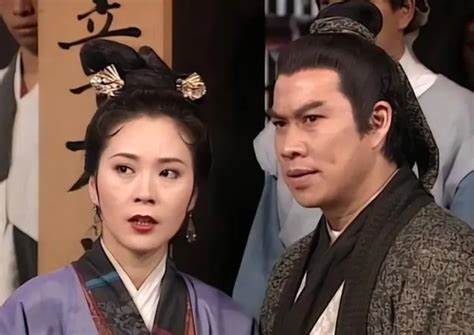
\includegraphics[width=0.7\linewidth]{黄蓉郭靖1}
		\caption{锁定仇人}
	\end{figure}
	
	\clearpage
	\begin{figure}[!htb]
		\centering
		\subfloat[]{
			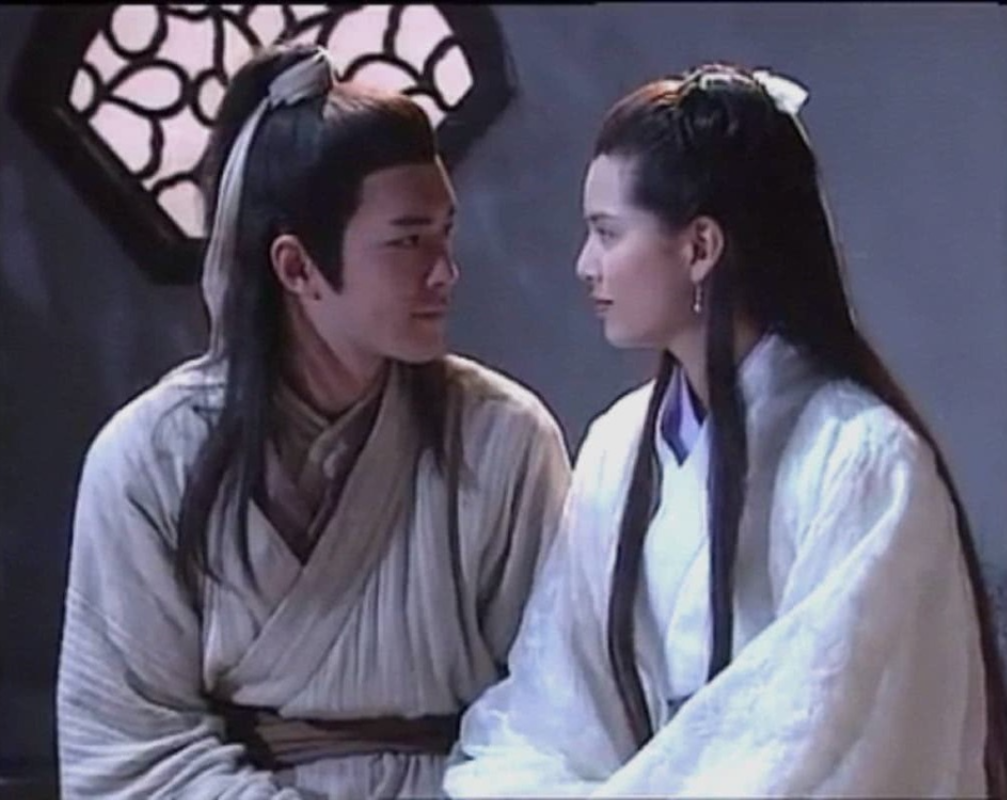
\includegraphics[width=0.4\linewidth]{杨过小龙女3}
			\label{fig: 见到姑姑嘻嘻}
		}
		\hfill
		\subfloat[]{
			
\includegraphics[width=0.4\linewidth]{杨过小龙女6}
			\label{fig: 姑姑见我不嘻嘻}
		}
		\caption[报仇哪有姑姑重要]{报仇哪有姑姑重要。\subref{fig: 见到姑姑嘻嘻}见到姑姑我嘻嘻;\subref{fig: 姑姑见我不嘻嘻}姑姑见我不嘻嘻} \label{fig: 报仇哪有姑姑重要}
	\end{figure}
	

	需要注意,图\ref{fig: 报仇哪有姑姑重要}中引用子图\ref{fig: 见到姑姑嘻嘻}和本段中引用子图使用的命令分别为\shad{$\backslash$subref\{fig: 见到姑姑嘻嘻\}}和\shad{$\backslash$ref\{fig: 报仇哪有姑姑重要\}},它们分别生成仅含带括号子图编号和完整子图编号的结果。
	
	另外,图\ref{fig: 报仇哪有姑姑重要}的图题包含了子图题文本,但生成的图目录中却只有主图题文本,其实现方式为在主图题命令中使用可选参数单独指定图目录中的显示文本:\shad{$\backslash$caption[报仇哪有姑姑重要]}
	
	\begin{figure}[!htb]
		\centering
		\subfloat[]{
			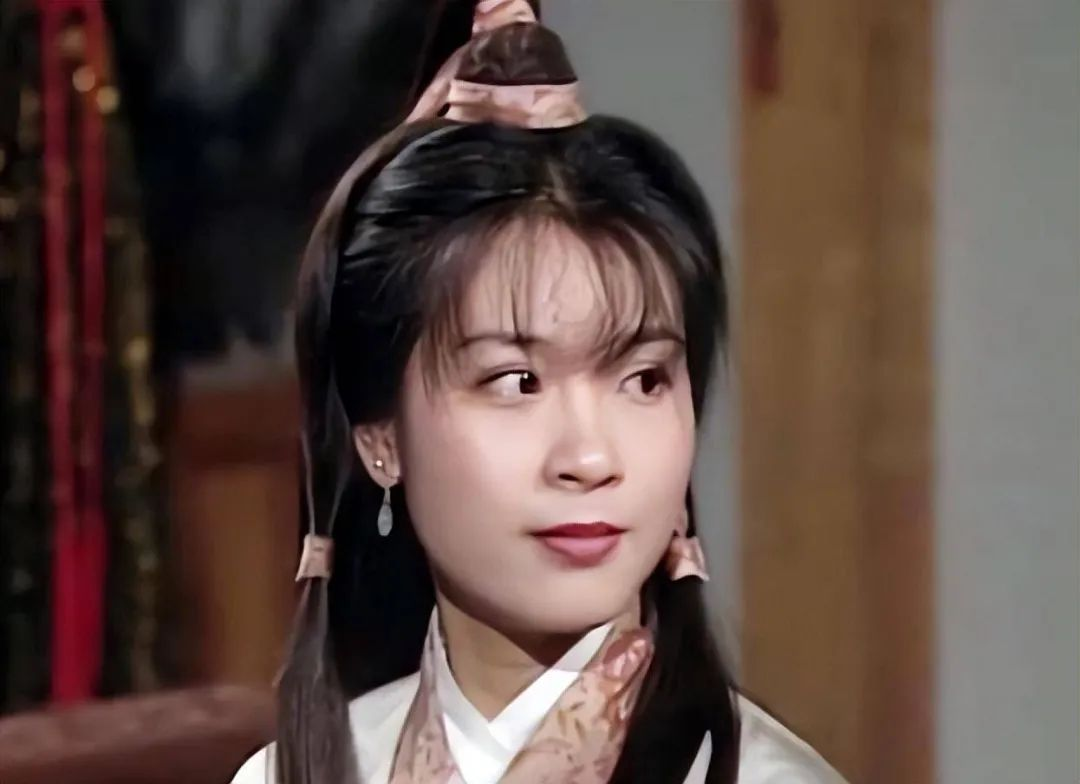
\includegraphics[width=0.4\linewidth]{陆无双2}
			\label{fig: 陆无双2}
		}
		\hfill
		\subfloat[]{
			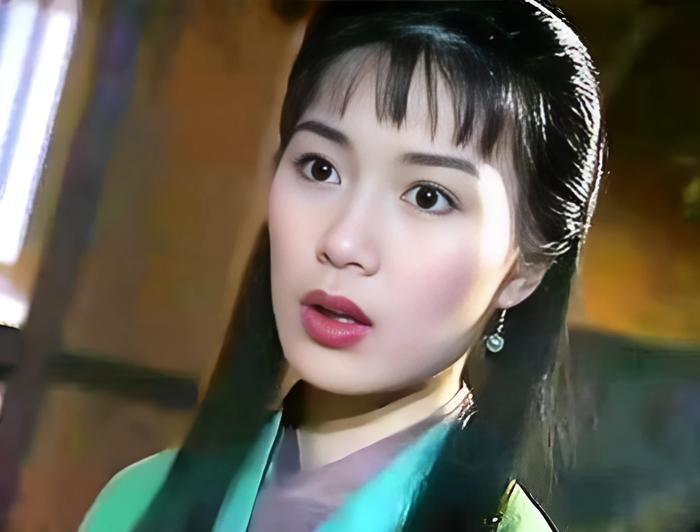
\includegraphics[width=0.4\linewidth]{程英3}
			\label{fig: 程英3}
		}
		\caption{找其他红颜知己嘻嘻。\subref{fig: 陆无双2}眼睛像姑姑;\subref{fig: 程英3}举止像姑姑} \label{fig: 红颜知己}
	\end{figure}
	
	\begin{figure}[!htb]
		\centering
		\subfloat[]{
			
\includegraphics[width=0.4\linewidth]{绿萼2}
			\label{fig: 绿萼2}
		}
		\hfill
		\subfloat[]{
			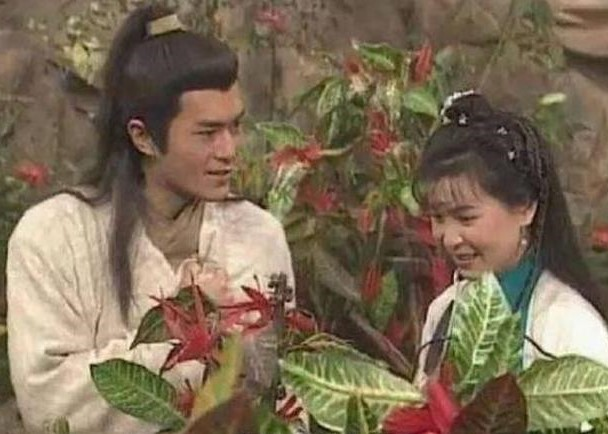
\includegraphics[width=0.4\linewidth]{杨过绿萼}
			\label{fig: 杨过绿萼}
		}
		\\
		\subfloat[]{
			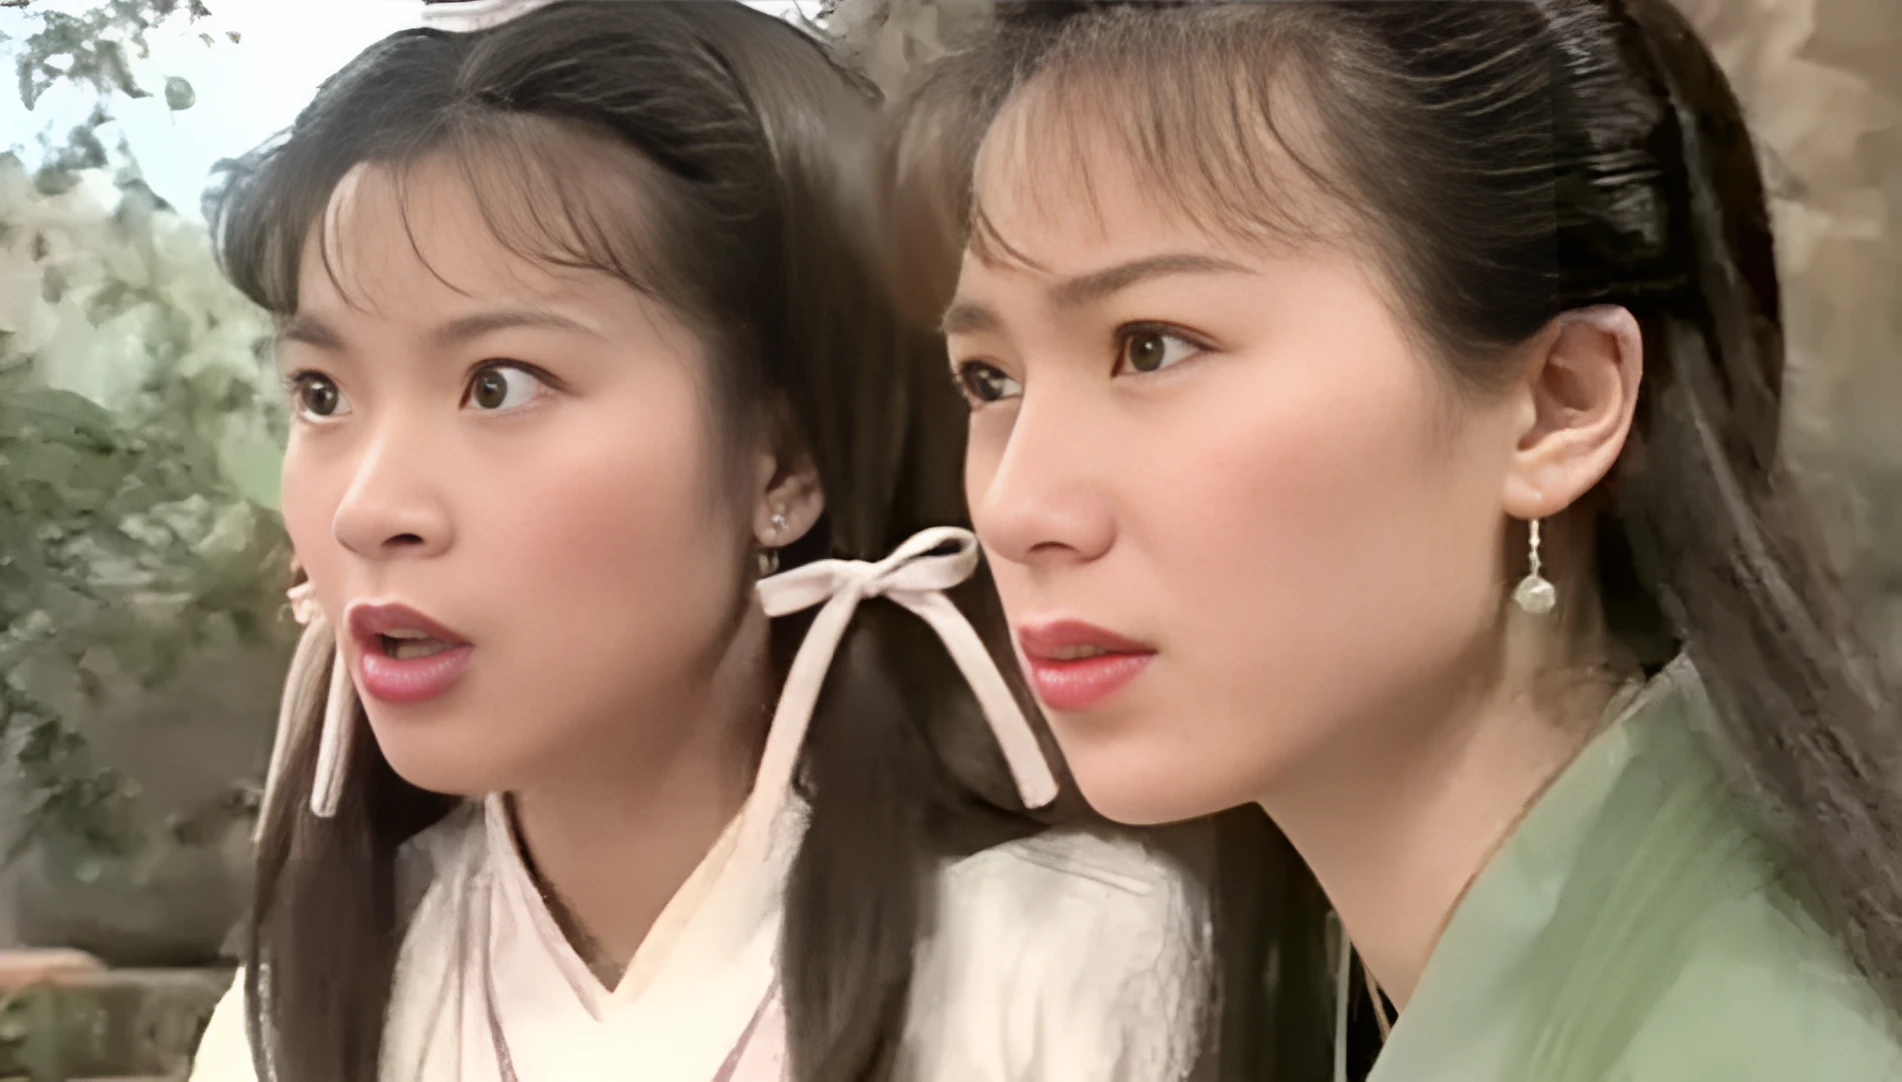
\includegraphics[width=\linewidth]{陆无双程英}
			\label{fig: GG}
		}
		\caption{撩妹是我杨过的被动技能。\subref{fig: 绿萼2}好腼腆的姑娘;\subref{fig: 杨过绿萼}你终于肯笑了;\subref{fig: GG}哦吼} \label{fig: 被动技能}
	\end{figure}
	
	\begin{figure}[!htb]
		\centering
		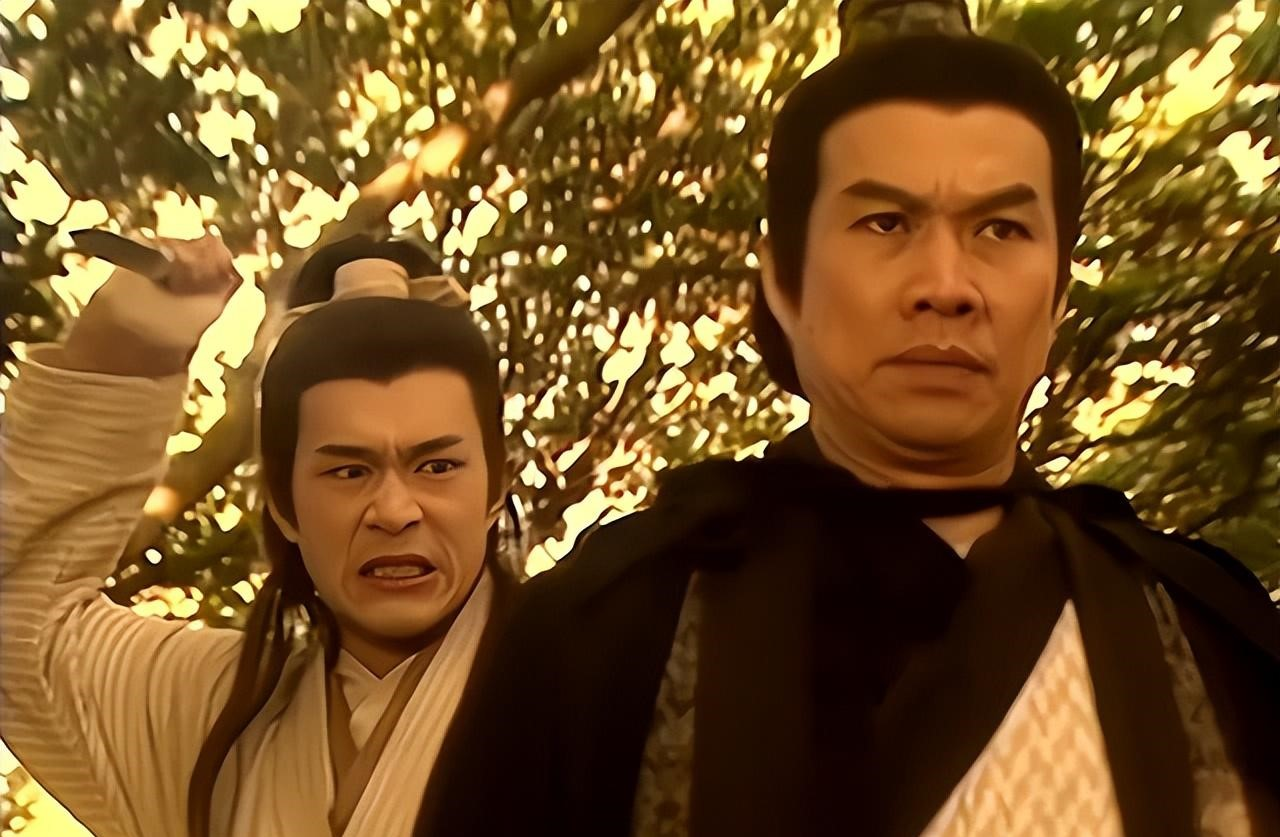
\includegraphics[width=0.9\linewidth]{杨过郭靖}
		\caption{还是推主线吧,动手动手}
	\end{figure}
	
	\clearpage
	\section{表格}
	
	表格的排版本身无需多言,使用\shad{table}+\shad{tabular}环境即可,但是要注意三线表中的三条线分别需要使用\shad{$\backslash$toprule}、\shad{$\backslash$midrule}、\shad{$\backslash$bottomrule}生成,这样才符合规范中对线宽的要求。注意不要用\shad{$\backslash$hline}。
	
	更需要说明的是生成带附注的表格。本模板采用\shad{threeparttable}宏包实现将表格中的附注内容顶格排版在表格底部:
	\begin{enumerate}
		\item 使用\shadcmd{tnote\{<label>\}}在表格中插入上标编号;
		\item 使用\shad{tablenotes}环境在表格底部排版附注。该环境提供选项\shad{online}用于将附注文本前的标号从默认的上标样式(见表\ref{tab: 江湖势力背调})更改为非上标样式(见表\ref{tab: 已习得武功})。
	\end{enumerate}
	
	\begin{table}[!ht]
		\caption{江湖势力背调} \label{tab: 江湖势力背调}
		\begin{threeparttable}
			\begin{tabular}{p{2cm} p{3cm} p{7cm}}
				\toprule
				\textbf{姓名} & \textbf{所属势力} & \textbf{武功绝学} \\
				\midrule
				郭靖 & 重阳宫 & 降龙十八掌 \\
				黄蓉 & 丐帮 & 打狗棒法 \\
				洪七公 & 丐帮 & 降龙十八掌、打狗棒法 \\
				黄老邪 & 桃花岛 & 弹指神通、落英神剑掌、玉箫剑法 \\
				老顽童 & 重阳宫 & 左右互博术\tnote{1} \\
				一灯 & 云南大理 & 一阳指\tnote{2}、千里传音 \\
				\bottomrule
			\end{tabular}
			\begin{tablenotes}
				\item[1] 自创武功
				\item[2] 云南大理段氏嫡传的武功,在点穴功夫中位居天下第一,运功后以右手食指点穴,出指可缓可快,缓时潇洒飘逸,快则疾如闪电,但着指之处,分毫不差。当与敌挣搏凶险之际,用此指法既可贴近径点敌人穴道,也可从远处欺近身去,一中即离,一攻而退,实为克敌保身的无上妙术。
			\end{tablenotes}
		\end{threeparttable}
	\end{table}
	
	\begin{table}[!ht]
		\caption{已习得武功} \label{tab: 已习得武功}
		\begin{threeparttable}
			\begin{tabular}{p{3cm} p{3cm} p{5cm}}
				\toprule
				\textbf{武功绝学} & \textbf{传授者} & \textbf{传授地点} \\
				\midrule
				蛤蟆功 & 欧阳锋 & 重阳山脉 \\
				九阴真经 & 小龙女 & 活死人墓 \\
				打狗棒法 & 洪七公、黄蓉 & 华山之巅、英雄大会 \\
				玉箫剑法 & 黄老邪 & 深山老林 \\
				黯然销魂掌\tnote{1} & 自创 & 海边 \\
				\bottomrule
			\end{tabular}
			\begin{tablenotes}[online]
				\item[1] 黯然销魂掌,是在杨过与小龙女离别后,认为今生再也见不到小龙女,悲从中来,由此创作了黯然销魂掌。黯然销魂掌和心情有关,此后杨过与小龙女重逢后,其心理愉悦,故使不出黯然销魂掌。
			\end{tablenotes}
		\end{threeparttable}
	\end{table}
	
	
	\clearpage
	\section{伪代码}
	
	伪代码基于\shad{algorithm2e}宏包提供的\shad{algorithm}环境,默认不添加左右侧框线,且顶部框线和底部框线类比规范对表格的要求进行了加粗,字体大小也调整到了\textbf{五号字},与表格保持一致。用户可以在载入文档类时添加\shad{boxruled}选项来恢复左右侧框线。该环境生成的伪码与正文文本保持相同宽度。
	
	除了\shad{algorithm2e}宏包本身提供的各种条件、循环语句,本模板基于宏包提供的接口,追加了\shad{Do While}和\shad{Loop}循环语句:
	\begin{itemize}
		\item \shadcmd{DoWhile(<紧跟关键字do的文本,可用于添加注释>)\{<循环条件>\}\{<循环体>\}}
		\item \shadcmd{Loop(<紧跟关键字loop的文本,可用于添加注释>)\{<循环体>\}}
	\end{itemize}
	
	
	此外,基于调整后的\shad{algorithm2e}环境,本模板进一步封装了\shad{algo}环境。从名字上可以看出,\shad{algo}环境比\shad{algorithm}环境生成的伪码浮动区域更\textbf{窄}。它除了接受浮动可选参数\shad{[htbp]},还提供了另一可选参数\shad{(<伪码距正文文本边界的总距离>)},该参数控制的是浮动体离正文文本边界的总距离,默认是\shad{4em},即单边缩进\shad{2em},与下方首行文本对齐。两种可选参数可以单独使用或同时使用,但要注意同时使用时的顺序必须与下方例子保持一致:
	
	\begin{verbatim}
		\begin{algo}[<浮动选项>](<伪码距正文文本边界的总距离>)
		    .....
		\end{algo}
	\end{verbatim}
	
	算法\ref{alg: algorithm环境伪码示例}和算法\ref{alg: algo环境伪码示例}分别展示了两种环境默认生成的伪码样式;过程\ref{alg: algorithm环境修改伪码标签示例}和过程\ref{alg: algo环境修改伪码标签并调整宽度示例}展示了如何修改伪码中的一些标签,以及调整\shad{alog}伪码宽度的具体做法。
	
	\begin{algorithm}[!h]
		\caption{algorithm环境伪码示例} \label{alg: algorithm环境伪码示例}
		\Input{1) 输入1;\newline 2) 输入2。}
		\Output{输出结果。}
		伪码行1。
		
		\For(\tcc*[f]{循环条件注释1}){循环条件1}{
			伪码行2。
			
			\tcp{注释2}
			伪码行3。
			
			\DoWhile(\tcc*[f]{循环条件注释3}){循环条件2}{
				伪码行4。
			}
			
			\tcc{loop循环}
			\Loop(\tcc*[f]{注释4}){
				循环体1。
			}
			
			\Repeat(\tcc*[f]{循环条件注释5}){循环条件3}{
				循环体2。
			}
			\eIf(\tcc*[f]{条件注释6}){条件语句6}{
				为真,伪码行5。
			}{
				条件为假,伪码行6。\tcp*[f]{repeat循环}
			}
			
			\If(\tcc*[f]{条件注释7}){条件语句7}{
				伪码行7。
			}
		}
		\textbf{return} 算法结果。
	\end{algorithm}
	
	\begin{algorithm}[!h]
		\renewcommand{\algorithmcfname}{过程}  % 修改伪码标签需要在\caption{}之前
		\caption{algorithm环境临时修改伪码标签示例} \label{alg: algorithm环境修改伪码标签示例}
		\SetKwInOut{Input}{In}
		\SetKwInOut{Output}{Out}
		\Input{1) 输入1; 2) 输入2。}
		\Output{输出结果。}
		伪码行1。
		
		\For(\tcc*[f]{循环条件注释1}){循环条件1}{
			伪码行2。
			
			\tcp{注释2}
			伪码行3。
			
			\DoWhile(\tcc*[f]{循环条件注释3}){循环条件2}{
				伪码行4。
			}
			
			\tcc{loop循环}
			\Loop(\tcc*[f]{注释4}){
				循环体1。
			}
			
			\Repeat(\tcc*[f]{循环条件注释5}){循环条件3}{
				循环体2。
			}
			\eIf(\tcc*[f]{条件注释6}){条件语句6}{
				为真,伪码行5。
			}{
				条件为假,伪码行6。\tcp*[f]{repeat循环}
			}
			
			\If(\tcc*[f]{条件注释7}){条件语句7}{
				伪码行7。
			}
		}
		\textbf{return} 算法结果。
	\end{algorithm}
	
	\begin{algo}[!h]
		\caption{algo环境伪码示例} \label{alg: algo环境伪码示例}
		\Input{1) 输入1;\newline 2) 输入2。}
		\Output{输出结果。}
		伪码行1。
		
		\For(\tcc*[f]{循环条件注释1}){循环条件1}{
			伪码行2。
			
			\tcp{注释2}
			伪码行3。
			
			\DoWhile(\tcc*[f]{循环条件注释3}){循环条件2}{
				伪码行4。
			}
			
			\tcc{loop循环}
			\Loop(\tcc*[f]{注释4}){
				循环体1。
			}
			
			\Repeat(\tcc*[f]{循环条件注释5}){循环条件3}{
				循环体2。
			}
			\eIf(\tcc*[f]{条件注释6}){条件语句6}{
				为真,伪码行5。
			}{
				条件为假,伪码行6。\tcp*[f]{repeat循环}
			}
			
			\If(\tcc*[f]{条件注释7}){条件语句7}{
				伪码行7。
			}
		}
		\textbf{return} 算法结果。
	\end{algo}
	
	\begin{algo}[!h](8em)
		\renewcommand{\algorithmcfname}{过程}  % 修改伪码标签需要在\caption{}之前
		\caption{algo环境临时修改伪码标签并调整宽度示例} \label{alg: algo环境修改伪码标签并调整宽度示例}
		\SetKwInOut{Input}{In}
		\SetKwInOut{Output}{Out}
		\Input{1) 输入1; 2) 输入2。}
		\Output{输出结果。}
		伪码行1。
		
		\For(\tcc*[f]{循环条件注释1}){循环条件1}{
			伪码行2。
			
			\tcp{注释2}
			伪码行3。
			
			\DoWhile(\tcc*[f]{循环条件注释3}){循环条件2}{
				伪码行4。
			}
			
			\tcc{loop循环}
			\Loop(\tcc*[f]{注释4}){
				循环体1。
			}
			
			\Repeat(\tcc*[f]{循环条件注释5}){循环条件3}{
				循环体2。
			}
			\eIf(\tcc*[f]{条件注释6}){条件语句6}{
				为真,伪码行5。
			}{
				条件为假,伪码行6。\tcp*[f]{repeat循环}
			}
			
			\If(\tcc*[f]{条件注释7}){条件语句7}{
				伪码行7。
			}
		}
		\textbf{return} 算法结果。
	\end{algo}
	
	\clearpage
	\section{定义、定理、命题、推论、引理、证明}
	
	本模板分别定义了环境:\shad{definition}、\shad{theorem}、\shad{proposition}、\shad{corollary}、\shad{lemma}和\shad{proof}。示例如下:
	
	\begin{definition}
		云南大理段氏嫡传的武功,在点穴功夫中位居天下第一,运功后以右手食指点穴,出指可缓可快,缓时潇洒飘逸,快则疾如闪电,但着指之处,分毫不差。当与敌挣搏凶险之际,用此指法既可贴近径点敌人穴道,也可从远处欺近身去,一中即离,一攻而退,实为克敌保身的无上妙术。
	\end{definition}
	
	\begin{theorem}
		云南大理段氏嫡传的武功,在点穴功夫中位居天下第一,运功后以右手食指点穴,出指可缓可快,缓时潇洒飘逸,快则疾如闪电,但着指之处,分毫不差。当与敌挣搏凶险之际,用此指法既可贴近径点敌人穴道,也可从远处欺近身去,一中即离,一攻而退,实为克敌保身的无上妙术。
	\end{theorem}
	
	\begin{proposition}
		云南大理段氏嫡传的武功,在点穴功夫中位居天下第一,运功后以右手食指点穴,出指可缓可快,缓时潇洒飘逸,快则疾如闪电,但着指之处,分毫不差。当与敌挣搏凶险之际,用此指法既可贴近径点敌人穴道,也可从远处欺近身去,一中即离,一攻而退,实为克敌保身的无上妙术。
	\end{proposition}
	
	\begin{corollary}
		云南大理段氏嫡传的武功,在点穴功夫中位居天下第一,运功后以右手食指点穴,出指可缓可快,缓时潇洒飘逸,快则疾如闪电,但着指之处,分毫不差。当与敌挣搏凶险之际,用此指法既可贴近径点敌人穴道,也可从远处欺近身去,一中即离,一攻而退,实为克敌保身的无上妙术。
	\end{corollary}
	
	\begin{lemma}
		云南大理段氏嫡传的武功,在点穴功夫中位居天下第一,运功后以右手食指点穴,出指可缓可快,缓时潇洒飘逸,快则疾如闪电,但着指之处,分毫不差。当与敌挣搏凶险之际,用此指法既可贴近径点敌人穴道,也可从远处欺近身去,一中即离,一攻而退,实为克敌保身的无上妙术。
	\end{lemma}
	
	\begin{proof}
		云南大理段氏嫡传的武功,在点穴功夫中位居天下第一,运功后以右手食指点穴,出指可缓可快,缓时潇洒飘逸,快则疾如闪电,但着指之处,分毫不差。当与敌挣搏凶险之际,用此指法既可贴近径点敌人穴道,也可从远处欺近身去,一中即离,一攻而退,实为克敌保身的无上妙术。
	\end{proof}
	
	
	\section{脚注}
	
	本模板使用包含了带圈数字的字体来替换LaTeX绘制的带圈数字,提供了充足的带圈编号数量,同时保证了带圈脚注编号足够优雅。
	
	在正文中加入脚注直接在需要放置脚注标签的位置使用\\\shadcmd{footnote\{<脚注内容>\}}即可。
	
	在其他环境中,如表格,则需要需要使用\shadcmd{footnotemark}配合\\\shadcmd{footnotetext\{<脚注文本>\}}。在需要放置脚注标签的位置使用\shadcmd{footnotemark},然后在环境外使用\shadcmd{footnotetext\{<脚注文本>\}}指明脚注内容\footnote{更详细的使用方法参考\href{https://blog.csdn.net/xovee/article/details/127563209}{\shad{LaTeX脚注}}}。
	
	
	\section{引用}
	
	对公式、图片、表格、伪码、定义、定理、命题、推论、引理、证明等编号的引用直接用\shadcmd{ref\{<编号label>\}}即可,其中需要带括号公式编号则使用\shadcmd{eqref\{<公式label>\}}。
	
	若要对子图题编号进行完整引用直接使用\shadcmd{ref\{<子图题标签>\}}即可,它将生成形如\shad{1-1(a)}的完整编号;反之,若只希望单独引用子图题编号,比如在图题结尾按编号添加子图题文本,则需要使用\shadcmd{subref\{<子图题标签>\}},它将生成形如\shad{(a)}的单独编号。
	
	对参考文献的行内引用直接使用\shadcmd{cite\{<参考文献label>\}},以上标形式引用则使用\shadcmd{citess\{<参考文献label>\}}。
	
	参考文献的引用是基于\shad{natbib}宏包实现的,单次引用多篇参考文献时会自动排序并压缩序号(如果可以的话)。
	
	
	\section{参考文献编译}
	
	本模板实现了规范中列举的\textbf{期刊论文}、\textbf{会议论文}、\textbf{专著}、\textbf{学位论文}、\textbf{报纸文章}、\textbf{报告}、\textbf{授权专利}、\textbf{标准}、\textbf{电子文献},共计9种文献类型的排版风格。
	
	本模板为这些文献类型定义的\shad{.bib}数据库条目\textbf{类型标识}分别为\shad{article}、\shad{inproceedings/conference}、\shad{book}、\shad{mastersthesis/phdthesis}、\shad{news}、\shad{report}、\shad{patent}、\shad{standard}、\shad{digital}。
	
	不同文档类型条目包含不同的域,下面列举了一些\href{https://gr.uestc.edu.cn/xiazai/114/3917}{研究生学位论文撰写规范}中用作示例的参考文献对应的\shad{.bib}数据库形式,完全覆盖上述9种文献类型:
	
	\begin{verbatim}
	@book{教育部国家语言文字工作委员2018,
	    author={教育部国家语言文字工作委员},
	    title={通用规范汉字},
	    address={北京},
	    publisher={语文出版社},
	    year={2018},
	    language={schinese},
	}
	
	@standard{学位论文编写规范555,
	    author={全国信息与文献标准化技术委员},
	    title={学位论文编写规范},
	    number={GB/T 7713.1-2006},
	    address={北京},
	    publisher={中国标准出版社},
	    year={2007},
	    pages={17--20},
	}
	
	@article{王晓琰2019关于连续出版会议论文著录格式的探讨,
	    title={关于连续出版会议论文著录格式的探讨},
	    author={王晓琰 and 殷建芳 and 王晓峰 and 邓迎 and 杨蕾},
	    journal={学报编辑丛论},
	    number={0},
	    year={2019},
	    pages={162--165},
	    language={schinese},
	}
	
	@article{hu2014domain,
	    title={Domain decomposition method based on integral equation for solution of
	    scattering from very thin, conducting cavity},
	    author={Hu, Jun and Zhao, Ran and Tian, Mi and Zhao, Huapeng and Jiang,
	    Ming and Wei, Xiang and Nie, Zai Ping},
	    journal={IEEE Transactions on Antennas and Propagation},
	    volume={62},
	    number={10},
	    pages={5344--5348},
	    year={2014},
	    publisher={IEEE}
	}
	
	@inproceedings{bergamasco2015adopting,
	    title={Adopting an unconstrained ray model in light-field cameras for 3d
	    shape reconstruction},
	    author={Bergamasco, Filippo and Albarelli, Andrea and Cosmo, Luca and Torsello,
	    Andrea and Rodola, Emanuele and Cremers, Daniel},
	    booktitle={IEEE Conference on Computer Vision and Pattern Recognition},
	    pages={3003--3012},
	    year={2015},
	    organization={Boston, USA}
	}
	
	@article{xue2024survey,
	    title={A survey of beam management for mmWave and THz communications
	    towards 6G},
	    author={Xue, Qing and Ji, Chengwang and Ma, Shaodan and Guo, Jiajia and Xu,
	    Yongjun and Chen, Qianbin and Zhang, Wei},
	    journal={IEEE Communications Surveys \& Tutorials},
	    year={2024},
	    pages={1--41},
	    publisher={IEEE}
	}
	
	@book{罗杰斯2011,
	    author={罗杰斯},
	    title={西方文明史:问题与源头},
	    translator={潘惠霞 and 魏婧 and 杨艳 and 汤玲},
	    edition={2},
	    address={大连},
	    publisher={东北财经大学出版社},
	    year={2011},
	    pages={1-353},
	    language={schinese},
	}
	
	@book{harrington1993field,
	    title={Field computation by moment methods},
	    author={Harrington, Roger F},
	    year={1993},
	    pages={76--112},
	    edition={3},
	    address={New York},
	    publisher={Wiley-IEEE Press}
	}
	
	@digital{电子文献1,
	    author={Deverell, W and gler, D},
	    title={A companion to California history},
	    type={M/OL},
	    modifydate={2013-11-15},
	    url={http://onlinelibrary.wiley.com/doi/.ch2/summary},
	    doi={10.1002/9781444305036},
	    address={New York},
	    publisher={John Wiley \& Sons},
	    year={2013},
	    pages={21-22},
	    citedate={2014-06-24},
	}
	
	@digital{电子文献2,
	    author={Clerc, M},
	    title={Discrete particle swarm optimization: a fuzzy combinatorial box},
	    type={EB/OL},
	    modifydate={2010-07-16},
	    url={http://clere.maurice.free.fr/pso/Fuzzy_Discrere_PSO/Fuzzy_DPSO.html},
	}
	
	@mastersthesis{陈念永2001毫米波细胞生物效应及抗肿瘤研究,
	    author={陈念永},
	    title={毫米波细胞生物效应及抗肿瘤研究},
	    address={成都},
	    school={电子科技大学},
	    year={2001},
	    pages={50--60},
	}
	
	@news{顾春20122,
	    author={顾春},
	    title={牢牢把握稳中求进的总基调},
	    publisher={人民日报},
	    year={2012},
	    month={03},
	    day={31},
	    number={3},
	}
	
	@report{冯西桥1997,
	    author={冯西桥},
	    title={核反应堆压力容器的{LBB}分析},
	    address={北京},
	    publisher={清华大学核能技术设计研究院},
	    year={1997},
	}
	
	@patent{肖珍新2012,
	    author={肖珍新},
	    title={一种新型排渣阀调节降温装置},
	    number={ZL201120085830.0},
	    year={2012},
	    month={04},
	    day={25},
	}
	\end{verbatim}
	
	这些\shad{.bib}数据依次编译后的结果见本文档中附上的参考文献列表,用户可对应查看。感兴趣的朋友可与\href{https://gr.uestc.edu.cn/xiazai/114/3917}{\shad{研究生学位论文撰写规范}}中给出的结果进行对比,看看是否做到了完全复刻。
	
	生成参考文献最耗费精力的是维护正确的\shad{ref.bib}数据库。在这之后,只需要在正文的对应位置使用以下两行代码即可插入完整的参考文献列表:
	\begin{verbatim}
		\bibliographystyle{DissertUESTC}
		\bibliography{ref}
	\end{verbatim}
	
	多说两句:
	\begin{itemize}
		\item 对于某些缺少非必要信息的文献,本模板提供的\shad{.bst}文件依然可以正确处理。比如\cite{王晓琰2019关于连续出版会议论文著录格式的探讨}这篇期刊论文缺少卷号,它仍能仅排版期号,这是符合规范的。再比如,文献\cite{电子文献2}比文献\cite{电子文献1}少了\textbf{出版地}、\textbf{出版者}等信息,依然能正常排版;但是注意,\cite{电子文献2}已经是这类文献的最简形式,不可再缺信息。
		
		\item 对中文参考文献,如果希望将它们的第四顺位及以后的作者显示为\shad{“等”},则必须要在它们的bib条目中加入\shad{language=\{\}}域,并将值设置为\shad{schinese}。这是文献编译引擎判断该条参考文献是否是中文的唯一依据。类似的,\cite{罗杰斯2011}中的\shad{“等译”}、\shad{“2版”}均靠设置\shad{language=\{schinese\}}实现。我的建议是,虽然\shad{language}域并非是强制添加的,但对于中文文献,最好将其添加进去。
		
		\item 对电子文献,其类型众多,因此需要用户通过\shad{type=\{\}}域显式指定,如文献\cite{电子文献1}和\cite{电子文献2};而对其他的文献类型,只要在\shad{@}符号后输入了正确的类型标识,对应的类型标签会自动生成,无需用户手动逐条添加。
	\end{itemize}
	
	
	\acknowledgement
	
	致谢内容
	
	
	%% 参考文献部分
%	\nocite{*}
	\bibliographystyle{DissertUESTC}
	\bibliography{ref}
	
	% 附录起始位置
	\appendix
	
	\chapter{九阴真经原本}
	\section{气沉丹田}
	
	\chapter{黯然销魂掌秘籍}
	\section{真气运转}
	
	\achievement
	
	\noindent\textbf{发表论文:}
	
	\begin{itemize}
	    \item {\textbf{作者1}, 作者2*, 作者3, 作者4. Domain decomposition method based on integral equation for solution of scattering from very thin, conducting cavity. \emph{IEEE Transactions on Antennas and Propagation}, 2014, 62(10): 5344--5348. (\textbf{CCF评级}, \underline{中科院分区}, IF: 98.8)}
	\end{itemize}
	
	\noindent\textbf{发明专利:}
	
	\begin{itemize}
		\item \textbf{作者1}, 作者2*, 作者3, 作者4。一种基于xxxxx的真气运转方法: ZL201120846830.0. 2023--02--20.
		
	\end{itemize}
	
	\noindent\textbf{参与项目:}
	
	\begin{itemize}
		\item 项目号. 项目名称. 项目级别, 2020.01--2022.12.
	\end{itemize}
\end{document}